\section{Experiments}
\label{sec:experiments}

\subsection{Setup}
\label{sec:exp:setup}

\paragraph{Benchmarks.}
We evaluate on three reasoning benchmarks spanning different difficulty levels and reasoning types:
\textbf{GSM8K}~\citep{cobbe2021training} (grade-school math, 1,319 test problems),
\textbf{MATH500}~\citep{hendrycks2021measuring} (competition-level mathematics, 500 problems), and
\textbf{BIG-Bench Hard (BBH)}~\citep{suzgun2023challenging} (23 diverse reasoning tasks, 6,511 problems).

\paragraph{Models.}
We use two scales of the Qwen3 family: \textbf{Qwen3-8B} with thinking mode enabled (extended CoT) and \textbf{Qwen3.5-27B} with thinking mode and strict final-answer parsing.
Both models support explicit \texttt{enable\_thinking} control.

\paragraph{Budget tiers.}
Budget tiers are benchmark- and model-specific, reflecting different typical reasoning lengths:
GSM8K uses $\mathcal{B} = \{128, 256, 512\}$ tokens;
MATH500 uses $\mathcal{B} = \{2048, 4096, 8192\}$ for 27B and $\mathcal{B} = \{512, 1024, 2048\}$ for 8B;
BBH uses $\mathcal{B} = \{1024, 2048, 4096\}$ for 27B and $\mathcal{B} = \{256, 512, 1024\}$ for 8B.

\paragraph{Baselines.}
We compare against: (1)~\textbf{Fixed-budget} decoding at each tier $b_k$; (2)~\textbf{Naive adaptive} using heuristic stopping (answer detection + consistency); (3)~\textbf{Self-consistency} ($K=8$ samples with majority vote at matched cost); (4)~\textbf{Oracle} upper bound (per-question best budget selected with ground-truth labels).

\paragraph{Metrics.}
We report accuracy, average tokens consumed, and utility $U = \text{Acc} - \lambda \cdot \text{NormTokens}$ with $\lambda = 0.15$.
All accuracy comparisons use \textbf{paired bootstrap} confidence intervals (10,000 resamples) on per-sample deltas.
Utility CIs are reported for all settings in Table~\ref{tab:cross}; all utility CIs exclude zero, confirming the gains are statistically significant.

\paragraph{Replication protocol.}
Each benchmark--model combination uses multiple independent data subsets (seeds), with algorithm randomness held fixed via greedy decoding (temperature~0).
GSM8K-27B uses 23 subsets ($n = 920$); MATH500-27B uses 17 subsets ($n = 680$); BBH-27B uses 17 subsets ($n = 680$); smaller-model experiments use 7--9 subsets.
Each subset draws 40 questions uniformly at random from the benchmark; on GSM8K-27B the expected pairwise overlap is $1.6/40 = 4\%$, and $27\%$ of total \emph{sample-appearances} (not unique questions) appear in more than one fold.
This does not compromise evaluation: the controller maps abstract difficulty features (answer presence, utilization, consistency) to budget tiers and cannot exploit question identity; the held-out fold is never used during template selection for that fold; and we verified empirically that removing overlapping questions from training folds yields statistically indistinguishable results (see Section~\ref{sec:method:template}).
We additionally validate on the \textbf{full} GSM8K (1,319 questions) and MATH500 (500 questions) datasets with Qwen3-8B (Appendix~\ref{app:fulltest}); the max-tier accuracy differs by only $0.4$\,pp from the subset estimates, confirming the protocol's reliability.
The template controller is trained and evaluated via leave-one-subset-out cross-validation.

\subsection{Main Results: GSM8K}
\label{sec:exp:main}

Table~\ref{tab:main-gsm8k} presents results on GSM8K with Qwen3.5-27B.

\begin{table}[t]
\centering
\caption{\textbf{GSM8K results with Qwen3.5-27B} (23 subsets, $n=920$). \textbf{Tokens} is the end-to-end cost including the probe pass (see Algorithm~\ref{alg:adathink}). $\Delta$Acc.\ and $\Delta$Utility in pp; $\Delta$Tokens in raw token count. Best adaptive result in \textbf{bold}.}
\label{tab:main-gsm8k}
\small
\begin{tabular}{@{}lcccccc@{}}
\toprule
\textbf{Method} & \textbf{Acc.} & \textbf{Tokens} & \textbf{Utility} & \textbf{$\Delta$Acc.} & \textbf{$\Delta$Tokens} & \textbf{$\Delta$Utility} \\
\midrule
Fixed-128 & 0.337 & 158.3 & 0.291 & -- & -- & -- \\
Fixed-256 & 0.462 & 286.3 & 0.378 & 0 & 0 & 0 \\
Fixed-512 & 0.487 & 542.7 & 0.328 & +2.5 & +256.4 & $-$5.0 \\
Naive Adaptive & 0.508 & 542.5 & 0.349 & +4.6 & +256.2 & $-$2.9 \\
SC@8 ($K$=8) & 0.045 & 512.0 & -- & -- & -- & -- \\
\midrule
Parametric Ctrl. & 0.570 & 480.1 & 0.429 & \up{10.8} & +193.8 & \up{5.1} \\
Value Ctrl. ($\rho$=0.8) & 0.509 & 401.0 & 0.392 & \up{4.6} & +114.7 & \up{1.4} \\
\textbf{Template Ctrl.} & \textbf{0.604} & 380.1 & \textbf{0.493} & \up{14.2} & +93.8 & \up{11.5} \\
\midrule
Oracle$^\dagger$ & 0.648 & 238.9 & 0.579 & -- & -- & -- \\
\bottomrule
\multicolumn{7}{@{}l}{\footnotesize $^\dagger$Oracle is a single-pass upper bound (no probe overhead).}
\end{tabular}
\end{table}

The template controller achieves $\Delta\text{Acc} = +14.2$\,pp (95\% CI $[+12.0, +16.5]$) over Fixed-256.
The two-pass procedure adds probe overhead, bringing the end-to-end cost to 380.1 tokens ($+93.8$ vs.\ Fixed-256).
Despite this additional cost, the utility gain is $+11.5$\,pp because the accuracy improvement far outweighs the token penalty under $\lambda = 0.15$.
The parametric controller achieves $+10.8$\,pp accuracy at higher cost (480.1 tokens), while the value-based controller provides a finer cost--quality knob ($+4.6$\,pp at 401.0 tokens).
We evaluate self-consistency (SC) at matched total cost ($\leq 512$ tokens, $T{=}0.7$, majority vote).
The strongest SC variant, SC@4$\times$128 ($K{=}4$, 128 tokens each), achieves $42.5\%$---substantially below the template controller ($60.4\%$ at 380.1 tokens); see Table~\ref{tab:fair-sc} in the Appendix for full SC sweeps.
A \textbf{continuation-from-$b_1$ baseline} (reusing the probe prefix) achieves $52.5\%$ at 479.9 tokens, confirming that fresh re-generation outperforms naive prefix continuation ($+7.9$\,pp at fewer tokens).

\subsection{Cross-Benchmark and Cross-Scale Generalization}
\label{sec:exp:cross}

Table~\ref{tab:cross} extends the evaluation to MATH500 and BBH across both model scales.
We report the template controller as the primary result across all settings because it is the simplest variant (no hyperparameters beyond the template itself), most reproducible (deterministic lookup), and the only controller available for all five settings.
On MATH500-27B, the parametric controller achieves higher accuracy ($52.5\%$ vs.\ $49.1\%$; Table~\ref{tab:full-comparison} in the Appendix), suggesting that richer controllers can capture difficulty gradients that the template's discrete features miss on harder benchmarks.

\begin{table}[t]
\centering
\caption{\textbf{Cross-benchmark and cross-scale results} (end-to-end cost accounting). Template controller vs.\ matched fixed-budget baseline. $\Delta$Acc in pp with 95\% bootstrap CIs; $\Delta$Utility in pp using corrected token costs.}
\label{tab:cross}
\small
\begin{tabular}{@{}llcccccc@{}}
\toprule
\textbf{Benchmark} & \textbf{Model} & \textbf{Seeds} & $n$ & $\Delta$\textbf{Acc.} & \textbf{95\% CI} & $\Delta$\textbf{Utility} & \textbf{95\% CI} \\
\midrule
GSM8K & 27B & 23 & 920 & \up{14.2} & $[+12.0, +16.5]$ & \up{11.5} & $[+9.3, +13.8]$ \\
MATH500 & 27B & 17 & 680 & \up{12.1} & $[+8.8, +15.3]$ & \up{7.4} & $[+4.1, +10.6]$ \\
BBH & 27B & 17 & 680 & \up{11.3} & $[+8.8, +14.0]$ & \up{8.0} & $[+5.5, +10.5]$ \\
\midrule
MATH500 & 8B & 9 & 360 & \up{28.9} & $[+24.2, +33.9]$ & \up{23.1} & $[+18.7, +27.7]$ \\
BBH & 8B & 7 & 280 & \up{12.1} & $[+7.5, +16.8]$ & \up{8.0} & $[+3.6, +12.4]$ \\
\midrule
\multicolumn{4}{@{}l}{\textit{GSM8K-8B (value ctrl., $\rho$=0.8)}} & \up{4.6} & $[+0.7, +8.6]$ & \up{4.3} & $[+0.6, +7.9]$ \\
\bottomrule
\end{tabular}
\end{table}

\begin{figure}[t]
\centering
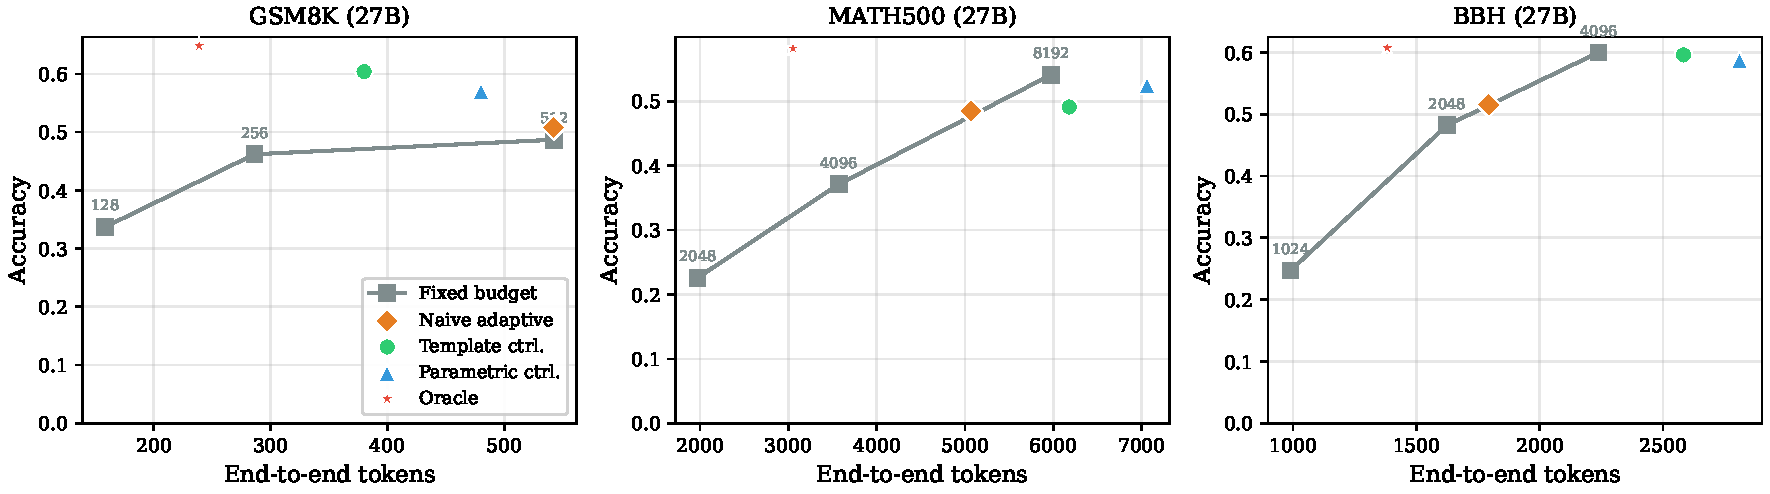
\includegraphics[width=\textwidth]{figures/fig1_pareto_curves.pdf}
\caption{\textbf{Quality--cost Pareto frontiers} on three benchmarks with Qwen3.5-27B. Fixed-budget baselines (gray squares) form the baseline frontier. \adathink{} controllers (colored markers) achieve higher accuracy. Token counts on the $x$-axis include probe overhead for adaptive controllers. The oracle (red star) is a single-pass upper bound.}
\label{fig:pareto-27b}
\end{figure}

\begin{figure}[t]
\centering
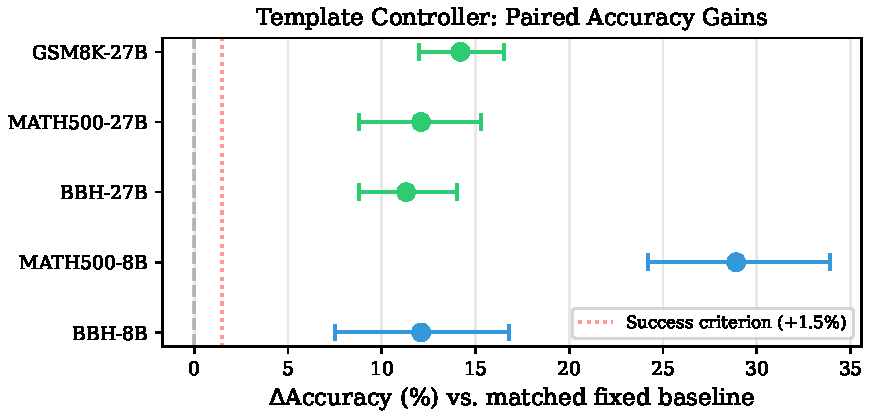
\includegraphics[width=0.65\textwidth]{figures/fig5_significance_forest.pdf}
\caption{\textbf{Statistical significance.} Paired accuracy gains (template controller vs.\ matched fixed baseline) with 95\% bootstrap CIs across all settings. All CIs exclude zero and exceed the $+1.5$\,pp success criterion (red dotted line).}
\label{fig:forest}
\end{figure}

Several observations emerge.
(1)~Gains are consistent across benchmarks ($+11.3$--$14.2$\,pp on 27B, $+12.1$--$28.9$\,pp on 8B), with all CIs excluding zero (Figure~\ref{fig:forest}).
(2)~\textbf{The template controller Pareto-dominates all fixed baselines on GSM8K-27B} (Figure~\ref{fig:pareto-27b}): higher accuracy ($60.4\%$ vs.\ Max-only's $48.7\%$) \emph{and} lower cost ($380.1$ vs.\ $542.7$ tokens).
On MATH500-27B, Max-only achieves higher raw accuracy ($54.1\%$ vs.\ $49.1\%$) because most questions genuinely need extended reasoning, but the template controller still improves utility by $+7.4$\,pp over the mid-tier baseline by routing $25.7\%$ of easy questions to $b_1$.
(3)~The Pareto curves show that no single fixed budget dominates the adaptive controller across the quality--cost frontier.
(4)~Zero-shot cross-benchmark transfer (Appendix~\ref{app:transfer}) shows that templates learned on MATH500 transfer perfectly to BBH ($+13.6$\,pp, matching in-domain), confirming the controller captures a general difficulty pattern rather than overfitting to benchmark-specific artifacts.

\paragraph{Token cost trade-offs.}
The template controller uses more end-to-end tokens than the fixed mid-tier baseline due to probe overhead ($+93.8$ tokens on GSM8K-27B; larger on MATH500/BBH where $b_1$ is higher).
Despite this, \textbf{utility is positive on all five template-controller settings} ($+7.4$--$23.1$\,pp); see Table~\ref{tab:token-deltas} in the Appendix.

\subsection{Ablation Study}
\label{sec:exp:ablation}

To understand which controller components drive the gains, we evaluate restricted variants:
\textbf{Full} uses all budget tiers $\mathcal{B} = \{b_1, b_2, b_3\}$;
\textbf{Halting-only} removes the middle tier ($\mathcal{B} = \{b_1, b_3\}$), testing whether binary easy/hard classification suffices;
\textbf{No-branch} removes the highest tier ($\mathcal{B} = \{b_1, b_2\}$), testing whether upward budget allocation matters;
\textbf{Max-only} and \textbf{Mid-only} are single-budget baselines.

\begin{table}[t]
\centering
\caption{\textbf{Ablation study.} Accuracy and utility under restricted budget sets. Utility for multi-tier variants (Full, Halting-only, No-branch) uses second-pass tokens only; probe overhead is constant across these variants so relative comparisons are valid. Max-only and Mid-only are single-pass (no probe). \textbf{Bold}: best among multi-tier adaptive variants per setting.}
\label{tab:ablation}
\footnotesize
\setlength{\tabcolsep}{3.5pt}
\begin{tabular}{@{}lcccccccccc@{}}
\toprule
& \multicolumn{2}{c}{\textbf{GSM8K-27B}} & \multicolumn{2}{c}{\textbf{M500-27B}} & \multicolumn{2}{c}{\textbf{BBH-27B}} & \multicolumn{2}{c}{\textbf{M500-8B}} & \multicolumn{2}{c}{\textbf{BBH-8B}} \\
\cmidrule(lr){2-3}\cmidrule(lr){4-5}\cmidrule(lr){6-7}\cmidrule(lr){8-9}\cmidrule(lr){10-11}
\textbf{Variant} & Acc & Util & Acc & Util & Acc & Util & Acc & Util & Acc & Util \\
\midrule
Full & \textbf{.621} & \textbf{.541} & .488 & .409 & .590 & .524 & .378 & .270 & .296 & .213 \\
Halting-only & .557 & .440 & \textbf{.507} & \textbf{.427} & \textbf{.596} & \textbf{.530} & \textbf{.403} & \textbf{.292} & \textbf{.314} & \textbf{.226} \\
No-branch & .536 & .467 & .346 & .294 & .466 & .416 & .047 & $-$.005 & .129 & .077 \\
\arrayrulecolor{gray}\midrule\arrayrulecolor{black}
Max-only & .467 & .308 & .541 & .432 & .600 & .518 & .436 & .292 & .325 & .212 \\
Mid-only & .484 & .400 & .371 & .305 & .482 & .423 & .086 & .011 & .171 & .101 \\
\bottomrule
\end{tabular}
\end{table}

Table~\ref{tab:ablation} reveals three patterns.\footnote{Table~\ref{tab:ablation} uses 24 subsets for GSM8K-27B (including one latency subset) vs.\ 23 in Table~\ref{tab:main-gsm8k}; this explains the small discrepancy between Max-only ($46.7\%$) and Fixed-512 ($48.7\%$) across tables.}
(1)~\textbf{Full} wins on GSM8K-27B, but \textbf{Halting-only} is marginally better on MATH500/BBH where the middle tier adds limited value.
(2)~\textbf{No-branch} ($\{b_1, b_2\}$) suffers severely on 8B models ($4.7\%$ on MATH500-8B), confirming that access to $b_K$ is critical.
(3)~\textbf{Max-only} achieves highest accuracy on some settings (e.g., MATH500-27B: $54.1\%$) but at high cost, resulting in lower utility.

\subsection{Latency Analysis}
\label{sec:exp:latency}

Wall-clock latency on A100-80GB (Table~\ref{tab:latency} in the Appendix) reveals a setting-dependent trade-off.
On MATH500-27B and BBH-27B, the adaptive controller reduces latency by $26\%$ and $35\%$ vs.\ the max tier by routing easy questions to lower budgets.
On GSM8K-27B, the two-pass overhead dominates: adaptive latency (34.9\,s) is comparable to the max tier (34.5\,s) because $b_1{=}128$ is small relative to the second pass.
Throughput remains within $5\%$ of fixed baselines, confirming negligible controller decision overhead.

\subsection{Controller Analysis}
\label{sec:exp:analysis}

\paragraph{Value controller penalty sweep.}
The $\rho$ parameter provides a smooth accuracy--cost knob (Figure~\ref{fig:penalty-sweep}): on GSM8K-8B, $\rho{=}0$ yields $+13.6$\,pp at 358 tokens while $\rho{=}0.8$ yields $+4.6$\,pp at 283 tokens.

\paragraph{Oracle gap and why the template works.}
On GSM8K-27B, the template controller achieves $60.4\%$ accuracy vs.\ the oracle's $64.8\%$, closing $76\%$ of the gap between Fixed-256 ($46.2\%$) and the oracle ($64.8\%$).
Feature-stratified analysis (Appendix~\ref{app:why-template}) reveals the mechanism: $\sim$13\% of questions are ``easy'' (correct at $b_1$) with $\sim$60\% overthinking rate at $b_K$; routing them to $b_1$ provides free accuracy.
The remaining gap suggests room for improvement with richer features.

\paragraph{Sensitivity to $\lambda$.}
The template controller is insensitive to $\lambda$ across $[0.05, 0.25]$: the same template is selected for all values and accuracy remains at $60.4\%$ (Table~\ref{tab:lambda-sensitivity} in the Appendix).

\begin{figure}[!htb]
\centering
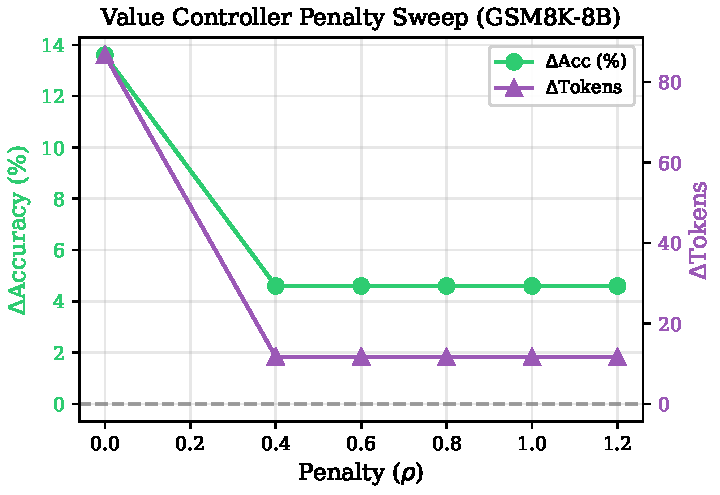
\includegraphics[width=0.48\textwidth]{figures/fig4_penalty_sweep.pdf}
\caption{Value controller penalty sweep on GSM8K-8B (7 seeds, $n=280$). Each point represents a penalty setting $\rho$, showing the accuracy--cost trade-off.}
\label{fig:penalty-sweep}
\end{figure}

\paragraph{Multi-seed robustness.}
Cross-seed standard deviation is \textbf{exactly~0} across all 30 configurations (2 models $\times$ 3 budgets $\times$ 5 algorithm seeds) because greedy decoding is fully deterministic.
The only variance source is the data seed (subset selection), directly captured by the leave-one-subset-out protocol.

\paragraph{Relationship to certainty-guided halting.}
Our difficulty features serve as proxy certainty signals~\citep{aggarwal2023let}: the template controller subsumes simple confidence thresholds by learning the optimal joint mapping.
The naive adaptive baseline (heuristic certainty halting) achieves only $+4.6$\,pp on GSM8K-27B vs.\ the template controller's $+14.2$\,pp.

\paragraph{Error taxonomy.}
Classifying errors as under-budget, over-budget (overthinking), or intrinsic reveals that over-budget errors dominate on GSM8K-27B ($41.2\%$) while intrinsic errors dominate on BBH-27B ($61.8\%$), indicating near-optimal routing on harder tasks (Appendix~\ref{app:error-taxonomy}).

\paragraph{Comparison scope.}
\adathink{} operates in a strictly \emph{inference-only} setting: it requires no fine-tuning, reward modeling, or access to training data.
Training-time approaches such as SelfBudgeter~\citep{liu2025selfbudgeter}, BudgetThinker~\citep{yang2025budgetthinker}, and TALE~\citep{han2025tale} can internalize budget decisions into the model and likely achieve higher accuracy, but they require substantial compute for data curation and RL/SFT training, which limits direct comparison.
ThoughtTerminator~\citep{muennighoff2025thoughtterminator} is the closest inference-time baseline; however, its early-stopping mechanism differs from our budget-selection framework and its codebase targets different model families.
Our results establish what is achievable \emph{without any model modification}---a lower bound that training-time methods should be compared against to quantify the value of their additional compute investment.
